\chapter{Classificação de Dados} \label{cap:classificação}

A classificação consiste em atribuir categorias a objetos ou dados e pode ser realizada por meio de inúmeras técnicas, as quais podem
ser divididas em dois tipos: supervisionada e não supervisionada. \cite{tan2013data, han2011data, clustering_review}.

Nas técnicas supervisionadas os objetos de dados são analisados a partir de rótulos de classe predefinidos nos objetos, ou seja, 
com as categorias previamente definidas e conhecidas. \citeonline{han2011data} chamam esse tipo de dado de ``dado treinado''
(aqueles cujos rótulos são conhecidos), onde o modelo que o descreve é obtido a partir da análise dos rótulos.

Na classificação não supervisionada, os rótulos de classe são obtidos a partir da análise dos dados dos objetos, tão somente \cite{tan2013data}.
A clusterização é uma das estratégias não supervisionadas mais conhecida e utilizada e demontra-se adequada para o contexto
do ``Empurrando Juntos'', no qual os grupos são formados com base em cada voto.

A clusterização foi denominada por \citeonline{clustering_review} como uma técnica para organização ou agrupamento em \textit{clusters} 
de uma coleção de elementos que sigam padrões baseado em similaridade.
\citeonline{tan2013data} definem a análise de \textit{clusters}, ou clusterização, como a ação que agrupa objetos de dados
baseada apenas nas informações contidas nos dados do próprio objeto que permitam descrever os objetos e suas relações. Um \textit{cluster}
então, pode ser visto como uma classe de objetos da qual é possível derivar regras para o grupo \cite{han2011data}.

Trata-se de uma técnica bastante utilizada em análise exploratórias, agrupamentos, 
tomada de decisão e implementações de aprendizado de máquina, como:
mineração de dados, recuperação de documentos, segmentação de imagens e padronização \cite{clustering_review}.

\citeonline{tan2013data, clustering_review} apresentam a clusterização dividida em alguns tipos: 
hierárquica ou particional; exclusiva, sobreposta ou \textit{fuzzy}; completa ou parcial.

\section{Tipos de clusterização}
Na clusterização particional o agrupamento dos 
objetos de dados é realizado em simples \textit{clusters}, o que significa que pertencem apenas a um \textit{cluster} \cite{tan2013data}.

\citeonline{clustering_review} definem uma clusterização hierárquica quando ela produz uma série
de partições aninhadas baseadas em um critério para junção ou separação dos \textit{clusters} por meio de similaridade. 
\citeonline{tan2013data} afirmam que esse tipo de clusterização acontece quando algoritmo
produz um resultado no qual é possível obter \textit{subclusters} e dessa forma os \textit{clusters} são aninhados
e organizados como uma árvore, seguindo a ideia de hierarquia.

No processo de clusterização, os objetos de dados podem pertencer a um único \textit{cluster} exclusivamente ou podem
pertencer a diferentes \textit{clusters} ao mesmo tempo. O primeiro caso é o que caracteriza uma clusterização exclusiva e o segundo caracteriza a sobreposta \cite{tan2013data}. 
Já o tipo \textit{fuzzy} trata da pertinência dos objetos a um grupo de forma probabilística, 
ou em um grau de pertinência, em vez de determinar se o objeto pertence ou não àquele grupo \cite{tan2013data, clustering_review}.

Por fim, \citeonline{tan2013data} definem uma clusterização como completa quando no resultado todos os objetos estão em pelo menos um grupo. 
Pois, na clusterização parcial alguns elementos podem ficar sem grupo caso não sejam compatíveis com algum \textit{cluster} formado.

\section{Passos para a clusterização}

Embora, cada tipo de clusterização tenha sua particularidade, para todos eles existem alguns passos necessários, apresentados na Figura \ref{fig:tasks_clustering}, 
para obter os dados classificados ao final do processo.

\begin{figure}[h]
\centering
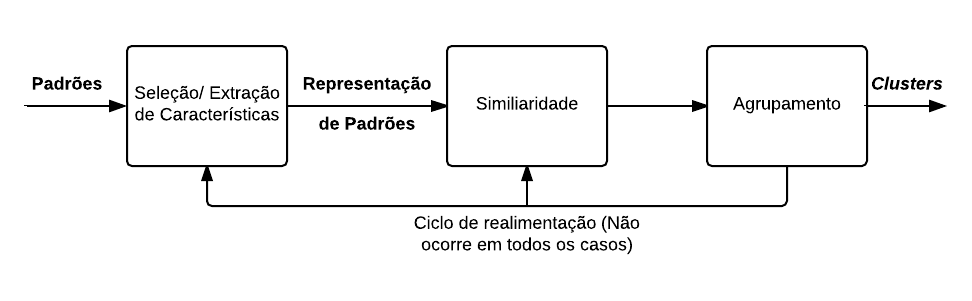
\includegraphics[scale=0.5]{figuras/tasks_clustering.png}
\caption{Passos para clusterização. Adaptado de \citeonline{clustering_review}}
\label{fig:tasks_clustering}
\end{figure}

O primeiro passo, seleção/extração de características tem como objetivo produzir o conjunto de objetos e dados a serem clusterizados. 
A seleção é o processo de identificação do subconjunto das características para ser utilizado na clusterização e 
a extração é o uso de uma ou mais transformações das características de entrada para 
torná-las mais efetivas para a clusterização \cite{clustering_review}.

A representação de padrões é o número de classes, número de padrões e o número, tipo e escala
das características disponíveis para a clusterização.
A similaridade é medida, em geral, por uma função de distância entre um par de objetos. Além disso, utiliza-se também
o conceito inverso de dissimilaridade para calcular o quanto objetos são diferentes. Essa função de distância pode variar de acordo 
com o contexto da aplicação e tipo dos dados \cite{clustering_review}. 

E por fim, o agrupamento pode ser realizado com uso de inúmeras técnicas e algoritmos diferentes \cite{clustering_review}.
Os objetos são agrupados (ou ``clusterizados'') buscando maximizar a similaridade intraclasse e minimizar a similaridade interclasse.
Em outras palavras, o objetivo é formar \textit{clusters} cujos elementos tenham alta similaridade entre si em um mesmo \textit{cluster} 
e baixa similaridade a elementos de outros \textit{clusters} \cite{han2011data}.

Apesar de parecer lógico e simples querer maximizar a similaridade intraclasse e minimizar a similaridade interclasse entre um conjunto de dados, 
\citeonline{tan2013data} exemplificam o quão difícil esta tarefa pode ser na Figura \ref{fig:clusters_difficulty}, onde temos um conjunto
de pontos (a) que pode ser agrupado de formas diferentes gerando quantidades diferentes de \textit{clusters} (b, c, d).

\begin{figure}[ht!]
\centering
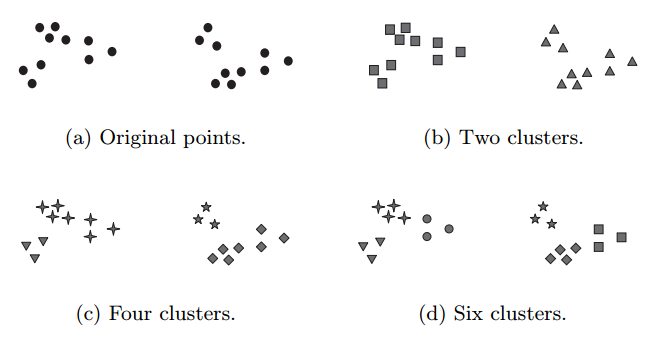
\includegraphics[scale=0.4]{figuras/clusters_difficulty.png}
\caption{Formas de se agrupar o mesmo conjunto de dados. Fonte: \cite{tan2013data}}
\label{fig:clusters_difficulty}
\end{figure}

Por isso para a construção de um algoritmo de clusterização deve-se definir, além do algoritmo principal a ser utilizado, as funções
de cálculo de similaridade e dissimilaridade para delimitação dos \textit{clusters}.

\section{Algoritmos de clusterização}
Conforme supracitado, existem diversos algoritmos criados para realizar a clusterização dos dados, que também são classificados em tipos
conforme os tipos de clusterização. A Figura \ref{fig:tipos_algoritmo} apresenta um esquemático dos tipos de algoritmos de clusterização de acordo
com as definições de \citeonline{gan2007data, han2011data, clustering_review}.

\begin{figure}[h!]
\centering
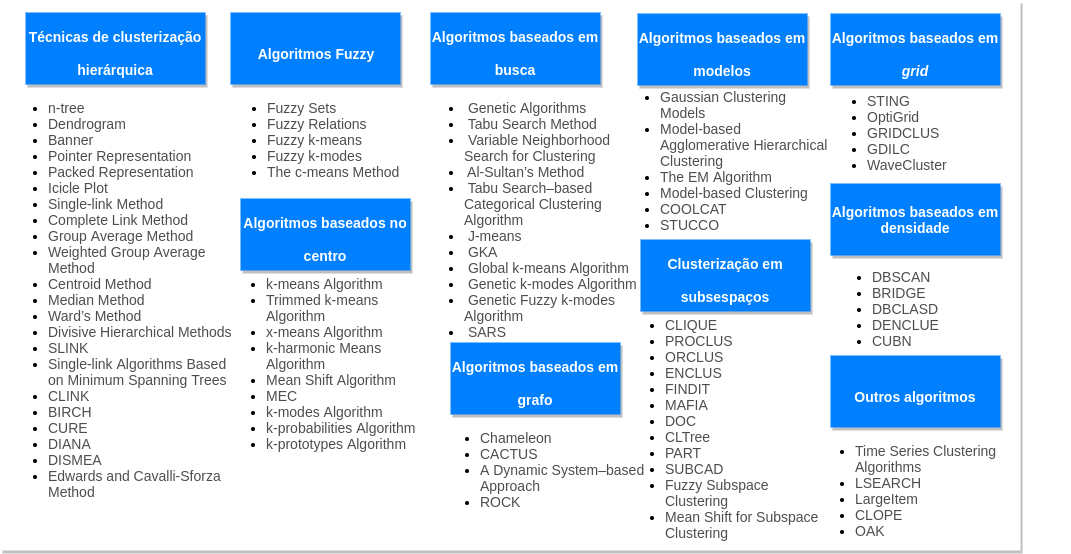
\includegraphics[scale=0.5]{figuras/algoritmos.png}
\caption{Algoritmos de clusterização}
\label{fig:tipos_algoritmo}
\end{figure}

A partir da figura apresentada, é notório que existe uma diversidade de algoritmos conhecidos. Neste trabalho, será descrito
apenas o algoritmo k-Means que foi escolhido como algoritmo de teste para o primeiro módulo do ``Empurrando Juntos'' e que de 
acordo com \citeonline{gan2007data, clustering_review}, é um dos mais utilizados.

\subsection*{k-Means}
O k-Means é um algoritmo particional e de clusterização exclusiva que forma $k$ \textit{clusters} a partir de $k$ centróides, onde $k$ é um número definido na aplicação 
\cite{clustering_review, tan2013data}. Um centróide é entendido, conceitualmente, como um ponto central \cite{han2011data}.

O algoritmo foi descrito por \citeonline{tan2013data} e \citeonline{han2011data} da seguinte forma:


\begin{center}
  \lstset{language=HTML, numbers=left, stepnumber=1}
  \begin{lstlisting}
  Escolha k pontos, dentro do conjunto de pontos a serem clusterizados ou não, como centróides iniciais
  Repita, até que os centróides não mudem:
    Forme k clusters de acordo com a menor distância dos pontos ao centróide, movendo os pontos para cada cluster.
    Recalcule o centróide de cada cluster baseado nos pontos do cluster.
  \end{lstlisting}
\end{center}


Nota-se que o número de centróides escolhidos determina a quantidade de \textit{clusters} no final do processamento.
Para o cálculo da distância entre os pontos podem ser utilizadas diversas técnicas. Contudo, é comum a utilização de um cálculo conhecido como distância Euclidiana, 
dado pela fórmula \ref{eq:euclidiana} \cite{clustering_review, tan2013data, han2011data}.

\begin{equation} \label{eq:euclidiana}
  d_{2}(x_i, x_j) = (\sum_{k=1}^{d} (x_{i,k} - x_{j,k})^2)^{1/2}
\end{equation}

A variação dentro do cluster é calculada pela fórmula \ref{eq:variacao}, na qual a 
função \textit{dist} representa a distância Euclidiana entre um ponto do
cluster e seu centróide. Ou seja, a variação é a soma dos quadrados
das distâncias de todos os pontos do cluster.

\begin{equation} \label{eq:variacao}
  E = \sum_{i=1}^{k} \sum_{p \epsilon C_{i}} dist(p, c_i)^2
\end{equation}

Na Figura \ref{fig:iteracoes_kmeans} é apresentada um exemplo das iterações utilizando o algoritmo descrito acima para um $k = 3$,
onde três pontos são escolhidos inicialmente como centróides e depois recalculados a cada iteração, gerando \textit{clusters} mais
refinados.

\begin{figure}[h!]
\centering
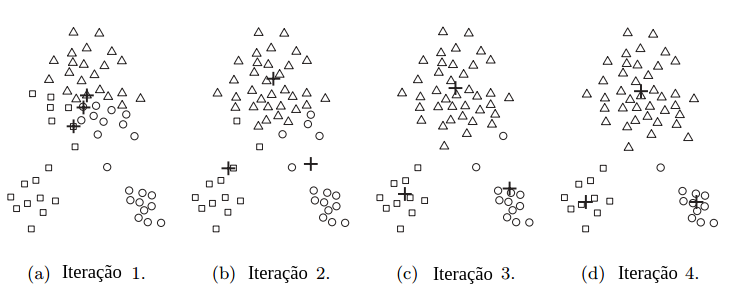
\includegraphics[scale=0.6]{figuras/iteracoes_kmeans.png}
\caption{Iterações de clusterização utilizando k-Means. Adaptado de \citeonline{tan2013data}}
\label{fig:iteracoes_kmeans}
\end{figure}

Na utilização do k-Means, definir previamente o valor de $k$, ou seja, o número de \textit{clusters} é considerada uma das desvantagens desse algoritmo. Todavia,
é possível contornar essa desvantagem escolhendo um intervalo de valores para execução do algoritmo e em seguida aplicar
uma técnica analítica para definir o melhor valor \cite{han2011data}.

% O algoritmo K-Means foi implementado em um módulo matemático em um trabalho anterior. O detalhamento do funcionamento do algoritmo
% para o módulo matemático e sua responsabilidade no fluxo do "Empurrando Juntos`` pode ser visto no Apêndice \ref{apd:kmeans}.

% \subsection{Métodos hierárquicos aglomerativos}
% 
% De acordo com \citeonline{tan2013data}, a categoria de técnicas de clusterização hierárquica é considerada a segunda mais 
% importante categoria. Os algoritmos de clusterização hierárquicos aglomerativos produzem um tipo de dendograma 
% com um agrupamento aninhado de padrões e níveis de similaridade \cite{han2011data, tan2013data}.  
% 
% Esse tipo de técnica trata, inicialmente, cada ponto como um \textit{cluster} e a cada passo mescla pares próximos de \textit{clusters}.
% Para isso, é definida a noção de proximidade destes grupos \cite{tan2013data}.
% 
% A depender das medidas de distância utilizadas, esses algoritmos podem ser subdivididos em técnicas específicas \cite{gan2007data}. 
% Nas subseções seguintes serão descritos alguns destes algoritmos.
% 
% \subsubsection*{Método de Ward}
% 
% Este algoritmo foi proposto por Ward Jr. e seu objetivo é realizar um procedimento de clusterização que minimize a perda 
% de informação associada a cada passo \cite{gan2007data}. Para isso, o algoritmo é baseada em alguma função objetiva, em geral, 
% o erro quadrados...
% 
% 
% \subsubsection*{Complete Link Method}
% 
% \subsubsection*{Group Average Method}
% 
% 
% \subsection{\textit{Density-Based Spatial Clustering of Applications with Noise}}
% O \textit{Density-Based Spatial Clustering of Applications with Noise} (DBSCAN) é um algoritmo baseado em densidade, 
% cuja abordagem é capaz de encontrar aleatoriamente \textit{clusters} definidos em regiões densas, separando os pontos
% em regiões de baixa densidade \cite{gan2007data}. Estes pontos de baixas densidade são classificados como ruídos (\textit{noise})
% e são omitidos no resultado final \cite{gan2007data, tan2013data}.
% 
% % Validar se é interessante falar sobre
% 
% \subsection{Birch}
% 
% \subsection{Gaussian Clustering models}